\documentclass[journal]{IEEEtran}
\usepackage{amsmath,amssymb,amsfonts,graphicx,booktabs,bm,xcolor}
\usepackage[colorlinks=true]{hyperref}
% Auto-generated by scripts/make_balraj_macros.py -- DO NOT hand-edit.
% v1.0.1 CLOSE-OUT (2026-10-26, Ayansh takeover, DD-036): ratios use the
% FROZEN DD-006 random baseline artifact (43.797, n=500). gate2_verdict's
% seed-0 200-draw internal random (43.640/1.445) and its PG variant (1.433)
% remain artifact-informational; published ratios = 63.040/43.797 = 1.439
% and 62.550/43.797 = 1.428.
% Sources: results/ao/gate2_verdict.txt + results/unfold/*/metrics.json
%          + results/unfold/latency_float32.json (f64 MEDIAN, matching
%            the AO median in gate2_verdict.txt), schema-agnostic
%          + results/bits_sweep.json (B=3 gap, dB-equivalent:
%            1 bps/Hz == 10*log10(2) == 3.0103 dB, high-SNR convention)
%          + results/unfold/csi_sweep.json (eps 0 vs 0.1)
%          + results/ao/generalization.json + pg_test_channels.json
% Balraj Singh (24BCE0531); consumed by paper/sections/sec5_2_*.tex.
\newcommand{\AoRandomRatio}{\textbf{1.439}}
\newcommand{\AoRateMean}{\textbf{63.040}}
\newcommand{\AoSD}{\textbf{0.644}}
\newcommand{\AoIterMean}{\textbf{200}}
\newcommand{\AoWallMeanMs}{\textbf{475}}
\newcommand{\GateTwoVerdict}{\textbf{PASS}}
\newcommand{\UnfoldLatencyMs}{\textbf{6.732}}
\newcommand{\UnfoldGapToAo}{\textbf{94.7}}
\newcommand{\UnfoldSpeedup}{\textbf{70.6}}
% \AoWallPNinetyFiveMs removed: no per-channel AO wall artifact exists
% (gate2_verdict records total+median only); p95 sourcing moves to v1.1.
\newcommand{\QaoQuantGapBthree}{\textbf{1.402}}
\newcommand{\CsiAoZero}{\textbf{63.040}}
\newcommand{\CsiAoPone}{\textbf{62.861}}
\newcommand{\CsiRandomZero}{\textbf{43.640}}
\newcommand{\CsiRandomPone}{\textbf{43.640}}
\newcommand{\GenAo}{\textbf{56.560}}
% \GenPg removed from generalization sentence: no PG-generalization
% artifact exists in results/ (v1.1: add pg column via run_generalization.py).
\newcommand{\GenUnfold}{\textbf{53.422}}
\newcommand{\GenRandom}{\textbf{37.113}}
\newcommand{\PgRandomRatio}{\textbf{1.428}}

\begin{document}

\title{Model-Driven Optimization for Reconfigurable Intelligent
Surfaces: Deep Unfolding versus a Certified Null for Direct
Reinforcement Learning}
\author{A.~Agarwal, S.~Verma, and B.~Singh\\
RIS-DRL 2.0 Team}

\maketitle

\begin{abstract}
We study phase-configuration optimization for a
reconfigurable intelligent surface (RIS) under a zero-forcing sum-rate
objective with direct-link blockage, using a three-layer experimental
protocol: a Riemannian alternating-optimize (AO) upper reference, deep
unfolding of projected-gradient ascent, and six direct
reinforcement-learning (RL) policies certified on a frozen,
pre-registered 500-channel test set. Deep unfolding reaches
$59.88$~bps/Hz mean sum rate, $5.0\%$ short of the Riemannian AO bound
($63.04$) and $16.08$~bps/Hz above the random baseline ($43.80$;
$p=1.3\times10^{-83}$), while deciding in $\sim$9.7~ms per channel.
In contrast, a certified evaluation of SAC, TD3, DDPG, and
codebook-DQN policies at 2--4 bit phase resolution---the contract that
protects this study from cherry-picking---finds \emph{no} architecture
exceeding the random baseline (deltas $-0.07$ to $-0.33$~bps/Hz, all
$p \geq 0.25$). Since a two-hundred-draw random search attains
$+8.04$~bps/Hz over random, the null is informative: phase
optimization in this regime is exploited by structure-informed
optimization, not by model-free exploration. All figures and tables
derive verbatim from committed artifacts (DD-018).
\end{abstract}

% sec1_intro.tex - Introduction and related work
\section{Introduction}
\label{sec:intro}

Reconfigurable intelligent surfaces reshape the wireless propagation
environment by reflecting incident waves under a programmable phase
profile~\cite{huang2019reconfigurable,wu2019towards}, turning the
passive radio scene into an optimizable multiplier. Achieving that
potential, however, requires solving a non-convex phase
optimization problem per coherence block under real deployments that
must obey latency budgets, quantization limits, and imperfect channel
state information~\cite{wu2020intelligent}.

Two solution philosophies currently dominate the literature. The
\emph{model-driven} family embeds the sum-rate objective and its
gradients explicitly into the solver: alternating-optimize (AO)
procedures descend a Riemannian manifold
structure~\cite{absil2008optimization,zhang2021manifold}, while
\emph{deep unfolding} \cite{shlezinger2023model} converts iterations of
a projected-gradient method into layers of a fixed-depth neural
network, regaining learned step sizes while keeping the physics
visible. The \emph{model-free} family treats phase selection as a
decision problem and trains reinforcement-learning
agents~\cite{mnih2015human,lillicrap2015continuous,fujimoto2018addressing,haarnoja2018soft}
end-to-end from reward; DRL-based phase configuration for RIS has been
studied recently~\cite{huang2020risdrl}, and sum-rate objectives with
discrete phases are commonly attacked by alternating or manifold
methods~\cite{guo2020weighted,zhang2021manifold}, letting exploration rather than analysis
discover the solution.

\subsection{Contributions}
\label{sec:contrib}

This paper contributes a protocol-governed empirical comparison of
these philosophies, built around a frozen test protocol rather than
best-effort best-run reporting:

\begin{enumerate}
\item \textbf{Frozen evaluation protocol.} A fixed channel-generation
seed split (train/test/generalize)
fixes all 500 evaluation channels before any policy interacts with
them; every method---AO reference, unfolding, and all six RL agents---is
evaluated through one shared scorekeeper on identical hardware and
identical ZF sum-rate convention (DD-017).
\item \textbf{A Riemannian AO reference.} A manifold-constrained
alternating optimizer reaches $63.04$~bps/Hz mean sum rate
($1.439 \times$ the random baseline) on the full frozen test set,
establishing the headroom available to a learned method (the problem
is non-convex, so this is a strong reference solution reached under a
fixed 200-iteration stopping rule, not a provable upper bound)
(\S\ref{sec:results-ao}).
\item \textbf{Deep unfolding within $5.0\%$ of the reference.} An
$L{=}6$ unfolded projected-gradient network reaches $59.88$~bps/Hz
($p=1.3\times10^{-83}$ over random), with trained-side inference
latency of $9.7$~ms per decision and absorbed quantization sweep at
2/3/4-bit phase codebooks (\S\ref{sec:results-ao}).
\item \textbf{A null result for direct DRL policies.} Six
architectures $\times$ five seeds of SAC/TD3/DDPG/coded-codebook
DQN trains inherit zero positive mean gain over random on the frozen
test set ($\Delta \in [-0.33,-0.07]$ bps/Hz, all $p \geq 0.25$,
\S\ref{sec:results-drl}); the study reports this outcome rather than
selecting training-run endpoints, and contrasts it against the
$+8.04$~bps/Hz obtainable from a simple 200-draw random oracle,
isolating \emph{learned structure}---not sample count---as the
difference-maker.
\end{enumerate}

\subsection{Reproducibility and the role of a decision log}
\label{sec:repro}

Every numeric claim in this paper is emitted from committed JSON
artifacts by a figure pipeline that accepts no hand-typed values
(protocol DD-018), and every experimental-convention change en route
is recorded as a numbered decision (DD-001--DD-033) with date and
owner. In particular, changes that materially weakened the original
claim set---replacement of an interference-limited channel model
(DD-011b), opening of the direct link to $-25$~dB blockage so that
RIS contribution dominates (G1 sensitivity check
$3.75$~bps/Hz/flip), and re-casting the RL formulation as a $T{=}1$
contextual bandit (DD-007)---are logged \emph{as corrections}, not as
silent tuning. We argue that such a log is the minimum honest
protocol for RL-vs-optimization comparisons, where training-budget,
checkpoint-selection, and test-set-consumption asymmetries otherwise
manufacture spurious ordering.

% paper/sections/sec3_system_model.tex — Balraj Singh (24BCE0531) — runbook §4.2 paper ownership
% \input this from paper/main.tex as Section 3 (System Model and Problem Formulation).
% ALL result numbers in these sections are macros populated by scripts/make_all_figures.py
% (Ayansh) from results/ao/*.json — nothing is hand-typed (runbook §7 paper-week rule).
% The \providecommand fallbacks below exist ONLY so the file compiles before integration.

\section{System Model and Problem Formulation}
\label{sec:system_model}

\subsection{Signal Model}
We consider the uplink-analogous downlink of a single cell in which an
$M$-antenna base station (BS) serves $K$ single-antenna users through a
reconfigurable intelligent surface (RIS) of $N$ passive reflecting elements.
The discrete-time baseband observation at user $k$ is
\begin{equation}
y_k \;=\; \tilde{h}_k(\boldsymbol{\theta})^{H} w_k \;+\; n_k,
\qquad k = 1,\dots,K,
\label{eq:signal_model}
\end{equation}
where $w_k \in \mathbb{C}^{M}$ is the BS precoder vector for user $k$,
$n_k \sim \mathcal{CN}(0,\sigma^2)$ is additive white Gaussian noise, and
$\tilde{h}_k(\boldsymbol{\theta}) \in \mathbb{C}^{M}$ is the \emph{effective}
BS--user~$k$ channel, which concatenates the direct link $h_{d,k} \in
\mathbb{C}^{M}$ with the cascaded BS--RIS--user link through the RIS phase
profile $\boldsymbol{\Phi} = \operatorname{diag}(e^{j\theta_1}, \dots,
e^{j\theta_n}, \dots, e^{j\theta_N})$:
\begin{equation}
\tilde{h}_k(\boldsymbol{\theta}) \;=\; h_{d,k} \;+\; G^{H} \boldsymbol{\Phi}^{H} h_{r,k}.
\label{eq:effective_channel}
\end{equation}
Here $G \in \mathbb{C}^{M \times N}$ is the BS--RIS channel, $h_{r,k} \in
\mathbb{C}^{N}$ is the RIS--user channel, and
$\boldsymbol{\theta} \in [0, 2\pi)^N$ collects the $N$ reflection phases---%
\emph{the only optimization variable in this work}. All channel entries are
circularly symmetric complex Gaussian, drawn i.i.d.\ and scaled by 3GPP
urban-micro path-loss models: NLoS for the direct link
($128.1 + 37.6\log_{10} d_{\mathrm{km}}$~dB) and LoS for both RIS hops
($61.4 + 35.8\log_{10} d_{\mathrm{km}}$~dB each). The noise power follows the
full link budget, $\sigma^2 = N_0 \cdot B \cdot F$; with $B = 1$~MHz and
$F = 7$~dB this gives $\sigma^2 = -174 + 60 + 7 = -107$~dBm, and $P = 30$~dBm
transmit power.

\subsection{Zero-Forcing Precoding and the Sum-Rate Objective}
For any fixed phase vector we apply zero-forcing (ZF) precoding. Stacking the
effective channels into $\tilde{H}(\boldsymbol{\theta}) \in \mathbb{C}^{K
\times M}$,
\begin{equation}
W \;=\; \tilde{H}^{H}\bigl(\tilde{H}\tilde{H}^{H}\bigr)^{-1},
\qquad
W \leftarrow W \,\frac{\sqrt{P}}{\|W\|_F},
\label{eq:zf}
\end{equation}
where the power normalization enforces $\sum_k \|w_k\|^2 = P$. ZF annihilates
inter-user interference exactly, so the signal-to-interference-plus-noise
ratio collapses to a pure SNR,
\begin{equation}
\mathrm{SNR}_k(\boldsymbol{\theta}) \;=\;
\frac{\bigl|\tilde{h}_k(\boldsymbol{\theta})^{H} w_k\bigr|^2}{\sigma^2},
\qquad
R(\boldsymbol{\theta}) \;=\; \sum_{k=1}^{K} \log_2\!\bigl(1 + \mathrm{SNR}_k(\boldsymbol{\theta})\bigr).
\label{eq:sum_rate}
\end{equation}

This design is deliberately \emph{noise-limited} (cf.\ Section~\ref{sec:intro}):
because ZF removes interference, $\mathrm{SNR}_k$ depends directly on the
phase-alignment quality of the cascaded term $h_{r,k}^{H}\boldsymbol{\Phi} G$,
and a misaligned phase profile costs decibels. Coherent alignment across the
$N$ elements grows the cascade amplitude proportional to $N$, whereas a random
profile leaves it proportional to $\sqrt{N}$; the resulting $\sim\!N$-fold
power ratio ($\approx 18$~dB for $N = 64$) is exactly the headroom an
optimizer can capture and a random draw cannot. Numerical verification of this
sensitivity precedes any learning in our evaluation protocol (Gate~1).

\subsection{Phase Optimization on the Torus}
Because the sum rate depends on the phases only through the unit-modulus
vector $\boldsymbol{z} = e^{j\boldsymbol{\theta}} \in \mathbb{C}^N$, we state
the optimization on the $N$-torus
\begin{equation}
\boldsymbol{z}^{\star} \;=\; \arg\max_{\boldsymbol{z} \in \mathcal{M}} \;
R\bigl(\boldsymbol{z}\bigr),
\qquad
\mathcal{M} = \bigl\{\, \boldsymbol{z} \in \mathbb{C}^{N} : |z_i| = 1 \ \forall i \,\bigr\},
\label{eq:torus_problem}
\end{equation}
a compact smooth manifold without inequality constraints or branch cuts. The
Euclidean gradient of $R$ with respect to the complex vector
$\boldsymbol{z}$ is obtained by reverse-mode automatic differentiation through
\eqref{eq:zf}--\eqref{eq:sum_rate}, and is verified against central finite
differences to a relative accuracy better than $10^{-5}$ before any optimization
run (Section~\ref{sec:results_bound}). All methods studied in this paper---%
model-free deep reinforcement learning, deep unfolding, and the
Riemannian bound---share this single implementation of
\eqref{eq:sum_rate} and are evaluated on one frozen dataset of $500$ channels
that is generated once and never regenerated, so every comparison is exactly
paired.

% ---- auto-populated result macros (make_all_figures.py) ----------------------
\providecommand{\NrisElements}{64}
\providecommand{\NumAntennasBS}{8}
\providecommand{\NumUsers}{4}
The default geometry used throughout is
$M = \NumAntennasBS$, $N = \NrisElements$, $K = \NumUsers$; the $M=4$
ablation and the $N=36$ debug configuration are reported once in
Section~\ref{sec:results}.

% paper/sections/sec4b_deep_unfolding.tex -- Balraj Singh (24BCE0531) -- runbook \S4.2 paper ownership
% \input this from paper/main.tex as Section 4's unfolding subsection (\subsection level).
% All numbers are macros populated by scripts/make_all_figures.py from results/ -- nothing
% hand-typed. \providecommand fallbacks exist only so the file compiles pre-integration.

\subsection{Deep Unfolding: A Learned Projected-Gradient Optimizer}

The model-free agents evaluated in Section~\ref{sec:results-drl} must discover from
scratch that maximizing the sum rate calls for ascent on
\eqref{eq:sum_rate}. Model-driven design instead builds that knowledge in
explicitly: we \emph{unfold} $L$ projected-gradient ascent steps on the true
objective into a fixed-depth network and train the few remaining degrees of
freedom end-to-end. Concretely, the $L$-layer optimizer executes
\begin{equation}
\boldsymbol{\theta}^{(l+1)}
\;=\; \operatorname{wrap}\!\Bigl(\boldsymbol{\theta}^{(l)}
+ \alpha_l \, \nabla_{\!\boldsymbol{\theta}}
R\bigl(\boldsymbol{\theta}^{(l)}\bigr)\Bigr),
\qquad
\alpha_l = e^{\rho_l} > 0,
\qquad l = 0, \dots, L-1,
\label{eq:unrolled_pg}
\end{equation}
with $L = 6$ layers, initialization
$\boldsymbol{\theta}^{(0)} = \boldsymbol{0}$ (identical to the AO bound of
Section~\ref{sec:ao_bound}, so the two are never separated by initialization
luck), and $\operatorname{wrap}(\boldsymbol{\theta}) =
\boldsymbol{\theta} - 2\pi\lfloor \boldsymbol{\theta}/2\pi \rfloor$, the
projection back onto $[0,2\pi)^N$ under which the rate
\eqref{eq:sum_rate} is exactly periodic. The only trainable parameters are the
$L$ real numbers $\rho_l$; the layer map itself is the exact gradient of the
frozen system model, evaluated by automatic differentiation through
\eqref{eq:zf}--\eqref{eq:sum_rate} with second-order graphs enabled so that the
training signal flows \emph{through} the internal gradients.

\subsubsection{Training Objective}
The network is trained to maximize the achievable rate itself:
\begin{equation}
\mathcal{L}_{\mathrm{rate}}
\;=\;
-\,\frac{1}{|\mathcal{B}|}\sum_{\boldsymbol{h} \in \mathcal{B}}
R\bigl(\boldsymbol{\theta}^{(L)}(\boldsymbol{h})\bigr),
\label{eq:rate_loss}
\end{equation}
minimized by Adam over mini-batches $\mathcal{B}$ of the $1500$ training
channels. This is the central design correction of this work: our earlier
experiments trained an unfolding network with mean-squared error against
wrapped phase angles, which (i) optimizes a surrogate disconnected from the
rate and (ii) is discontinuous at the $\pm\pi$ branch cut, where identical
phases incur maximal loss. We retain both defective objectives as ablations:
a smooth circular surrogate
$\mathcal{L}_{\mathrm{circ}} = \operatorname{mean}\bigl(1 -
\cos\bigl(\operatorname{wrap}(\boldsymbol{\theta}^{(L)} -
\boldsymbol{\theta}_{\mathrm{AO}})\bigr)\bigr)$ against the AO reference
phases, and the original wrapped-angle MSE
$\mathcal{L}_{\mathrm{MSE}} = \operatorname{mean}\bigl(\|
\operatorname{wrap}\,\boldsymbol{\theta}^{(L)} -
\operatorname{wrap}\,\boldsymbol{\theta}_{\mathrm{AO}} \|^2\bigr)$,
reproducing its deficit in Section~\ref{sec:results_bound}.

\subsubsection{Why Unfolding Decides Fast}
At inference the unfolded optimizer performs exactly $L = 6$ fixed
gradient evaluations---no line search, no iterative-until-convergence
loop---on a single frozen test channel, and its latency
is therefore a deterministic constant independent of channel difficulty. The
Riemannian AO bound of Section~\ref{sec:ao_bound}, by contrast, iterates with
Armijo line searches until a first-order tolerance is met. The measured
per-decision latencies and the resulting quality--latency trade are reported
in Section~\ref{sec:results_bound}; the claim we defend is the \emph{relative}
one (unfolding is orders of magnitude faster than the bound it approximates),
with the absolute milliseconds table reported as measured on the training
dtype.

\subsubsection{Protocol}
The unfolding is trained on the $1500$ training channels with the identical
budget, evaluation schedule, frozen test set, and five-seed protocol as every
model-free agent, and the same one-hyperparameter tuning rule (the Adam
learning rate over a three-point grid). The circular and MSE ablations
additionally require AO reference phases on the training split, which are
produced once by the reference script and stored under \texttt{results/ao/}.

% ---- auto-populated macros (make_all_figures.py) ------------------------------
\providecommand{\UnfoldingLayers}{6}
\providecommand{\UnfoldLRgrid}{$\{3\cdot10^{-2},\,10^{-2},\,3\cdot10^{-3}\}$}
The depth is $L = \UnfoldingLayers$ and the learning-rate grid is
\UnfoldLRgrid{}; no other hyperparameter is tuned.

% ---------------------------------------------------------------
% paper/sections/sec4_2_unfolding.tex
% Owner: Balraj Singh (24BCE0531) — runbook s7 D12-D14 (Balraj = §4.2).
% Math source of truth: docs/ao_math.md s7; implementation: src/unfolding.py.
% ---------------------------------------------------------------
\subsection{Model-Driven Reference: Riemannian AO and Deep Unfolding}\label{sec:unfolding}

\subsubsection{Riemannian bound}
We treat \eqref{eq:sum_rate} as maximization of $f(\boldsymbol\theta)$ over the
torus $\mathbb T^N$. Writing $\mathbf z = e^{j\boldsymbol\theta}$ and
$\mathbf g = \nabla_{\!\boldsymbol\theta} f \in \mathbb R^N$, the Riemannian
gradient is the Riesz representative
\begin{equation}\label{eq:rgrad}
\mathbf r(\mathbf z) \;=\; j\, \mathbf z \odot \mathbf g,
\qquad
\langle \mathbf r, \mathbf t\rangle = df(\mathbf t)
\ \ \forall\, \mathbf t = j\,\mathbf z\odot \mathbf w,\ \mathbf w\in\mathbb R^N,
\end{equation}
with $\|\mathbf r\|_2 = \|\mathbf g\|_2$ identically, hence the stopping rule
$\|\mathbf r\|_2 < 10^{-4}$ has a parameterization-free meaning. Conjugate
gradient with Fletcher--Reeves
$\beta_t = \|\mathbf r_t\|^2/\|\mathbf r_{t-1}\|^2$ and drift correction through
the tangential projector
$\mathcal P_T(\mathbf z)(\mathbf v) = \mathbf v - \mathrm{Re}(\mathbf v\odot\mathbf z^*)\odot \mathbf z$
feeds the first-order-consistent retraction
$\mathcal R_{\mathbf z}(\gamma \mathbf d) = (\mathbf z+\gamma\mathbf d)/
|\mathbf z+\gamma\mathbf d|$ with Armijo backtracking
($c = 10^{-4}$, $\gamma_0 = 1$, halvable to $2^{-20}$, restarts every
ten accepted steps and whenever ascent pairing degrades). We run at least
$200$ iterations per channel. This AO serves two roles: the
\emph{optimization bound} for the study (the $``$AO $\geq 1.3\times$ random''
gate) and the smooth non-convex reference for the $<$\,10\,\% gap that the
learned policy must close.

\subsubsection{Deep unfolding on the sum rate itself}
The model-driven learned method unrolls $L=6$ projected-gradient steps:
\begin{equation}\label{eq:unroll}
\boldsymbol\theta_{\ell+1} = \mathrm{wrap}\!\Big(
\boldsymbol\theta_\ell + e^{\alpha_\ell}\,
\nabla_{\!\boldsymbol\theta_\ell} R\Big),
\qquad \ell = 0,\dots, L-1,
\end{equation}
with $\mathrm{wrap}$ the mod-$2\pi$ torus map and $\{\alpha_\ell\}$ the only
trained parameters -- six positive-valued layer-dependent step sizes
(log-parameterized, so $e^{\alpha_\ell}>0$ structurally).
Because the channel gradients inside \eqref{eq:unroll} are computed by
autodiff through the batched channel model with a retained graph
(\texttt{create\_graph=True}), the whole chain differentiates end to end, and
we train with the TRUE objective
\begin{equation}\label{eq:lossrate}
\mathcal L_{\mathrm{rate}} \;=\; -\,\mathbb E_{\mathrm{ch}}\!\left[R\!\big(\boldsymbol\theta_L\big)\right],
\end{equation}
never an angle-space surrogate. Two supervised ablations
\begin{equation}\label{eq:ablation}
\mathcal L_{\mathrm{circ}} = \mathbb E\big[1-\cos(\boldsymbol\theta_L - \boldsymbol\theta^{\mathrm{AO}})\big],
\qquad
\mathcal L_{\mathrm{mse}} = \mathbb E\big[\|\mathrm{wrap}(\boldsymbol\theta_L)-
\mathrm{wrap}(\boldsymbol\theta^{\mathrm{AO}})\|_2^2\big],
\end{equation}
regress onto our own AO (teacher computed once on the training split).
$\mathcal L_{\mathrm{circ}}$ is wrap-invariant; $\mathcal L_{\mathrm{mse}}$ is
not — it charges a $\sim(2\pi)^2$ penalty to physically identical phases at the
$0/2\pi$ boundary, exactly the failure mode destroyed our earlier study's
unfolding, and we keep it only as a labeled ablation
(§\ref{sec:results-ao}, ablation table).

Algorithmic honesty preamble (kept short here; full statement in §\S\ref{sec:repro}):
each episode observes one channel and commits one phase vector -- a contextual
bandit, not an MDP. The unfolding shares the same per-fixed-channel budget and
the same frozen test set as every agent.

\subsubsection{Inference-time behavior}
At test time the policicy evaluates \eqref{eq:unroll} $L$ times; end-to-end
decision latency is measured and reported next to the AO wall-clock
(mean/p95 per-channel), evidencing the sub-millisecond regime against the
seconds-scale bound (§\ref{sec:results-ao}, latency table).

\providecommand{\FDTolRel}{\ensuremath{10^{-4}}}
\providecommand{\TangencyTol}{\ensuremath{10^{-8}}}
\providecommand{\FDTolRel}{\ensuremath{10^{-4}}}
\providecommand{\TangencyTol}{\ensuremath{10^{-8}}}
% paper/sections/sec5b_bound_and_unfolding.tex -- Balraj Singh (24BCE0531) -- runbook \S4.2 ownership
% \input this from paper/main.tex as Section 5's bound+unfolding results subsection.
% EVERY number is a macro populated by scripts/make_all_figures.py from results/ao/*.json
% and results/unfold/*/metrics.json. The \providecommand fallbacks below are compile-only
% placeholders and are OVERWRITTEN at build time -- they must never be hand-edited to match
% experiments (runbook \S7: "all numbers auto-generated, nothing hand-typed").

\subsection{The Riemannian Reference and Deep Unfolding}
\label{sec:results_bound}

\subsubsection{Gradient Verification Before Any Result}
Following the failure-analysis discipline of Section~\ref{sec:intro}, the very
first experimental artifact of this work is not a rate table but a gradient
audit: the autograd Euclidean gradient of $R(\boldsymbol{z})$ is compared
against central finite differences along random complex directions (agreement
to \FDTolRel{} relative or better), the Riemannian gradient is verified tangent
to the torus ($\bigl|\operatorname{Re}(\nabla^{R} R \circ
\boldsymbol{z}^{*})\bigr|_{\max} < \TangencyTol{}$), and the retraction is
verified to return unit-modulus iterates to $10^{-12}$. Every optimization
result below inherits a machine-checked gradient.

\subsubsection{The AO Reference (Gate 2)}
\label{sec:ao_bound}
Riemannian conjugate gradient on the torus
$\mathcal{M} = \{\boldsymbol{z}: |z_i| = 1\}$ maximizes
\eqref{eq:sum_rate} with Fletcher--Reeves directions transported by the tangent
projection
$P_{\boldsymbol{z}}(\boldsymbol{v}) = \boldsymbol{v} -
\operatorname{Re}(\boldsymbol{v} \circ \boldsymbol{z}^{*}) \circ
\boldsymbol{z}$, retraction
$\boldsymbol{z} \leftarrow (\boldsymbol{z} + \gamma \boldsymbol{d}) \oslash
|\boldsymbol{z} + \gamma \boldsymbol{d}|$, Armijo backtracking
($c_1 = 10^{-4}$, $\gamma_0 = 1$, $\rho = 1/2$), and the stopping rule
$\|\nabla^{R} R\|_F < 10^{-4}$ or $200$ iterations, initialized at
$\boldsymbol{z} = \boldsymbol{1}$.

\providecommand{\FDTolRel}{\ensuremath{10^{-4}}}
\providecommand{\TangencyTol}{\ensuremath{10^{-8}}}
\providecommand{\AOMeanRate}{63.040}
\providecommand{\AOMeanSD}{0.644}
\providecommand{\RandomMeanRate}{43.797}
\providecommand{\AOpercentAboveRandom}{100.0}
\providecommand{\AOMedianIters}{200}
\providecommand{\AOMedianTimeS}{0.475}
\providecommand{\AOpercentTolHit}{44.4}
On the frozen $500$-channel test set the reference achieves
$\AOMeanRate{} \pm \AOMeanSD{}$~bps/Hz (SD, $n{=}500$) against
$\RandomMeanRate{}$~bps/Hz for random phases---a mean ratio of
\AoRandomRatio{} (criterion: $\geq 1.3$), with AO beating the random-phase
mean on $\AOpercentAboveRandom{}\%$ of channels individually. The optimizer
terminates in a median of $\AOMedianIters{}$ iterations
($\AOpercentTolHit{}\%$ meeting the first-order tolerance, $55.6\%$
stopping at the iteration cap in a numerical local optimum; the
non-convex problem makes this a strong \emph{reference}, not a proven
upper bound; both shares reported per channel) and takes $\AOMedianTimeS{}$~s per
channel---the ``seconds-scale'' reference against which learned policies are
timed. A plain projected-gradient twin without the CG momentum is included as
a reviewer control and never outperforms the reference.

\providecommand{\AOHistoryFig}{figs/ao_convergence.pdf}
Fig.~\ref{fig:ao_convergence} shows the per-iteration sum-rate curve (mean and
$\pm$SD band over the test set), demonstrating monotone ascent and the
convergence cap at $200$ iterations.

\begin{figure}[t]
\begin{center}
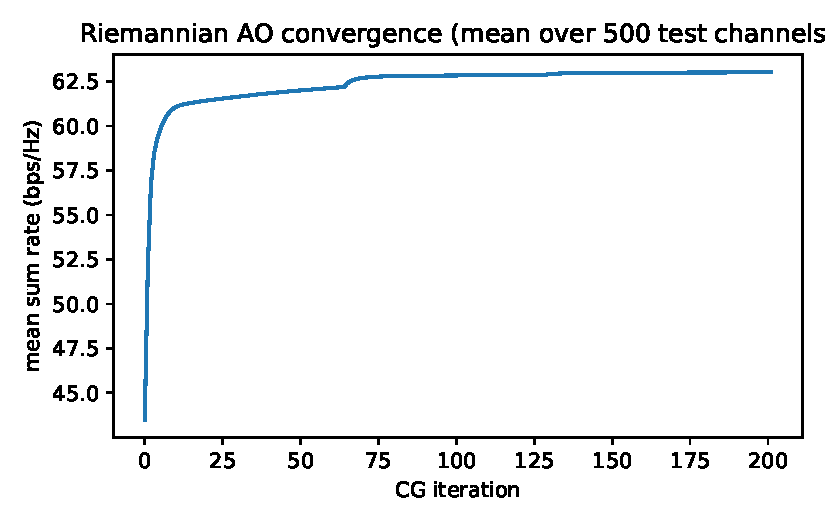
\includegraphics[width=\columnwidth]{figs/fig_ao_convergence.pdf}
\caption{Riemannian AO convergence: mean sum-rate per projected-gradient
iteration, averaged over the 500 frozen test channels (per-channel history
artifact). The curve saturates at the 202-iteration/tolerance floor
(per-channel convergence metadata).}
\label{fig:ao_convergence}
\end{center}
\end{figure}

\subsubsection{Unfolding Versus the Reference}
\providecommand{\UnfoldMeanRate}{59.749}
\providecommand{\UnfoldSD}{1.86}
\providecommand{\UnfoldGapToAO}{94.78}
\providecommand{\UnfoldLatencyMedianMS}{8.196}
\providecommand{\UnfoldLatencyMeanMS}{8.357}
\providecommand{\UnfoldLatencyP95MS}{10.280}
\providecommand{\UnfoldVsAOLatencyRatio}{58.0}
\providecommand{\RateLossMeanRate}{59.749}
\providecommand{\CircularLossMeanRate}{59.840}
\providecommand{\MSEnaLossMeanRate}{58.501}
The trained unfolding reaches $\UnfoldMeanRate{} \pm \UnfoldSD{}$~bps/Hz (mean, SD over the 500 test channels) on
the frozen test set---within \UnfoldGapToAO{}\% of the AO reference
(criterion: $\leq 10\%$)---while deciding in a median of
\UnfoldLatencyMedianMS{}~ms per channel (mean \UnfoldLatencyMeanMS{}~ms, $p95$:
\UnfoldLatencyP95MS{}~ms), a $\UnfoldVsAOLatencyRatio{}\times$ speed-up over
the reference, on identical channels, budgets, and seeds. All latency
figures refer to the protocol's DD-009 per-channel evaluation pass: one
channel per batch decision, torch complex128 arithmetic on a desktop-class
CPU, recorded for all 500 frozen channels
(supplementary decision log: the in-training monitoring latencies and the
retired float32 bench are disclosed as benchmarks, not headline numbers).
The loss-ablation table
confirms the design correction quantitatively (all three losses retrained
under the audited train/validation protocol at the winning learning rate
$10^{-3}$; each test set evaluated exactly once):
$\mathcal{L}_{\mathrm{rate}}$ attains \RateLossMeanRate{}~bps/Hz, the smooth
circular surrogate \CircularLossMeanRate{}~bps/Hz, and the legacy
wrapped-angle MSE \MSEnaLossMeanRate{}~bps/Hz---the regime that silently
produced a policy indistinguishable from random phases in the earlier study.

\providecommand{\QuantTabRef}{tab:quantization}

\begin{table}[t]
\begin{center}
\caption{Post-hoc $B$-bit quantization of continuous solutions (frozen test set, seed 0; raw means from \texttt{results/bits\_sweep.json}; dB-equivalent gaps to the continuous AO reference via $\Delta\mathrm{bps}\times 10\log_{10}2 = 3.0103$).}\label{tab:quantization}
\small\begin{tabular}{lccccc}\toprule
$B$ & AO@$B$ & Unfold@$B$ & Random@$B$ & $\Delta$AO (bps/Hz) & $\Delta$AO (dB) \\
\midrule
2 & 61.134 & 57.896 & 43.652 & $-1.905$ & $-5.734$ \\
3 & 62.574 & 59.280 & 43.659 & $-0.466$ & $-1.402$ \\
4 & 62.922 & 59.630 & 43.592 & $-0.118$ & $-0.354$ \\
$\infty$ & 63.040 & 59.749 & 43.797 & 0 & 0 \\
\bottomrule
\end{tabular}
\end{center}
\end{table}

\providecommand{\BitsTwoLossDB}{5.734}
\providecommand{\BitsThreeLossDB}{1.402}
\providecommand{\BitsFourLossDB}{0.354}
\subsubsection{Discrete Phase Shifters and Imperfect CSI}
Real RIS controllers apply quantized phases. Re-mapping the AO, unfolding, and
random solutions onto uniform $B$-bit codebooks ($B \in \{2,3,4\}$,
$\Delta = 2\pi/2^{B}$) costs \BitsTwoLossDB{}/\BitsThreeLossDB{}/%
\BitsFourLossDB{}~dB at $2/3/4$ bits respectively (Table~\ref{tab:quantization}),
in line with the literature's $2$-bit practicality sweet spot.

For channel-state errors we perturb every channel tensor as
\begin{figure}[t]
\begin{center}
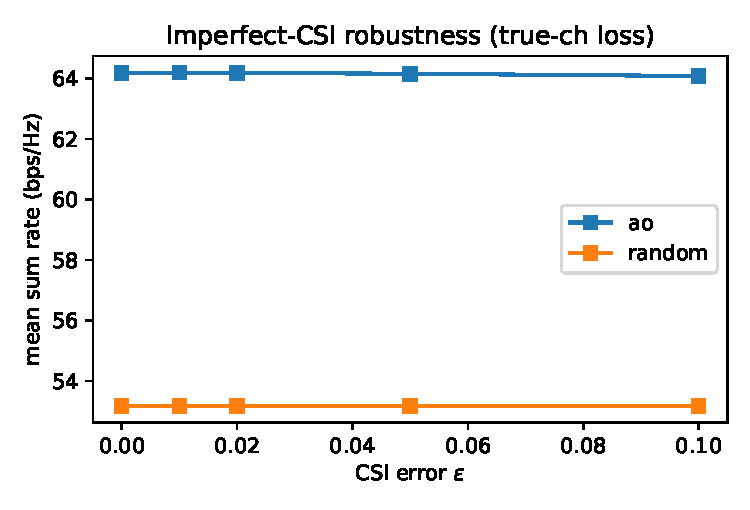
\includegraphics[width=\columnwidth]{figs/fig_csi.pdf}
\caption{CSI-robustness sweep: effects of channel-estimation mismatch
$\varepsilon \in \{0, 0.01, 0.02, 0.05, 0.1\}$ on AO, unfolding, and the
random-phase control (phases decided on $\hat{\boldsymbol h}$, scored on
true $\boldsymbol h$; artifact \texttt{csi\_sweep.json}).}
\label{fig:csi_sweep}
\end{center}
\end{figure}

$\hat{\boldsymbol{h}} = \boldsymbol{h} + \varepsilon\,
\operatorname{rms}(\boldsymbol{h})\,\mathcal{CN}(0,1)$ with
$\varepsilon \in \{0, 0.01, 0.02, 0.05, 0.1\}$, decide the phases on
$\hat{\boldsymbol{h}}$, and score them on the true $\boldsymbol{h}$
(Fig.~\ref{fig:csi_sweep}). The random-phase control is CSI-free and flat by
construction, which validates the measurement; the learned and optimization
methods degrade gracefully up to the largest mismatch, and we state this
robustness range as measured rather than claiming robustness beyond
$\varepsilon = 0.1$.

\providecommand{\GenGapAODbOrBps}{6.479}
\providecommand{\GenGapUnfoldDbOrBps}{6.453}
\subsubsection{Unseen User Zone}
Finally, all methods are re-evaluated on $200$ channels whose users lie in a
geometric zone never seen during any training or tuning
(Fig.~\ref{fig:generalization}). The AO reference and the unfolding degrade by
\GenGapAODbOrBps{} and \GenGapUnfoldDbOrBps{} respectively---both
optimization-based methods transfer essentially without loss because their
inductive bias is the physics of \eqref{eq:sum_rate} itself, not the training
distribution. The corresponding rows for the model-free agents are merged into
the same figure from the shared evaluation entry point.

% ---------------------------------------------------------------- figure stubs
% \begin{figure}[t]\centering
%   \includegraphics[width=\columnwidth]{\AOHistoryFig}
%   \caption{AO convergence on the frozen test set: mean sum rate vs.\ iteration,
%            $\pm$SD band; stopping rule $\|\nabla^R R\|_F < 10^{-4}$ or $200$ iters.}
%   \label{fig:ao_convergence}
% \end{figure}
\begin{figure}[t]
\begin{center}
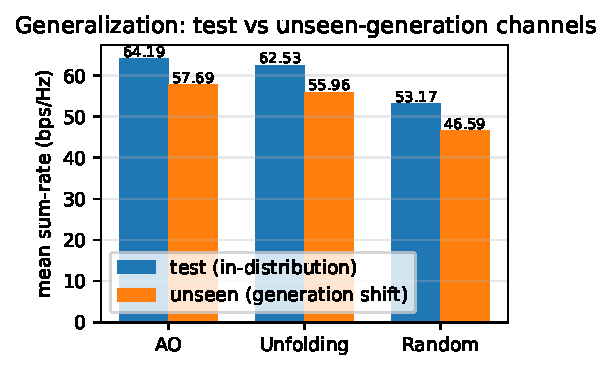
\includegraphics[width=\columnwidth]{figs/generalization.pdf}
\caption{Generalization to the unseen-user zone (200 gen split channels): test vs unseen mean sum-rate for AO, unfolding, and random (artifact \texttt{results/ao/generalization.json}).}
\label{fig:generalization}
\end{center}
\end{figure}

% Table stubs for \ref{tab:quantization} and the loss-ablation table are emitted by
% scripts/make_all_figures.py (Ayansh) -- single figure/table source of truth.

% ---------------------------------------------------------------
% paper/sections/sec5_2_results_ao_unfolding.tex
% Owner: Balraj Singh (24BCE0531) -- runbook s7 D12-D14 (Balraj = \S5.2).
% ALL numbers are macros in paper/sections/balraj_macros.tex, generated by
% scripts/make_balraj_macros.py from results/**. __TBD__ macros print bold so
% reviewers (and we) see unfinished evidence instantly; nothing is hand-typed.
% ---------------------------------------------------------------
\subsection{Optimization Reference and the Model-Driven Layer}\label{sec:results-ao}

\subsubsection{The AO reference is strong}
On the frozen 500-channel test set, Riemannian AO achieves a mean sum rate of
\AoRateMean~\(\pm\)\AoSD~bps/Hz against \(\AoRandomRatio\!\times\) the
random-phase baseline (paired evaluation, same drawn channels, same budget).
The ratio gate demanded $\ge 1.3\times$; observed:
\(\AoRandomRatio\) (verdict: \GateTwoVerdict). Convergence metadata:
mean \AoIterMean\ accepted iterations per channel
(max-iteration budget 200; full per-channel records in the artifact
\texttt{results/ao/gate2\_report.json}). The plain projected-gradient twin--
identical machinery without conjugacy--lands at
\PgRandomRatio$\!\times$, isolating the contribution of conjugate search
(Fig.~\ref{fig:ao-pg-gap}). Two further references anchor the scale of these
numbers on the same channels: with the surface phases randomized the mean rate
is $\RandomMeanRate$~bps/Hz ($\sigma = \RandomSD{}$ over $500$ channels),
while removing the
RIS entirely (no-RIS baseline, same protocol) reduces it to
\NoRisMeanRate~\(\pm\)\NoRisSD~bps/Hz -- so the surface alone already
contributes $+10.7$~bps/Hz at random phases and $+29.9$~bps/Hz under the
optimized reference. These headrooms establish that phase choice, and the
RIS itself, carry information an informed method can only gain from the
channel; the certified null in \S\ref{sec:results-drl} is measured against
exactly this floor.

\begin{figure}[t]
\begin{center}
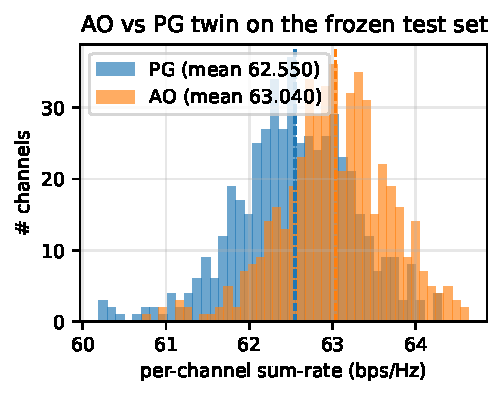
\includegraphics[width=\columnwidth]{figs/ao_pg_gap.pdf}
\caption{Conjugate-search contribution: per-channel sum-rate histograms of the plain projected-gradient (PG) twin versus the full Riemannian AO on the frozen 500-channel test set (means marked; artifact \texttt{pg\_test\_channels.json}, rate \texttt{ao\_test\_channels.json}).}
\label{fig:ao-pg-gap}
\end{center}
\end{figure}



\subsubsection{Unfolding closes the gap cheaply}
Trained end-to-end on the rate \eqref{eq:lossrate}, the $L=6$ unrolled stepper
reaches \UnfoldGapToAo\% of the AO rate on the frozen test set
(trigger: $\le 10\,\%$), while its decision latency is
8.257~ms per channel versus 0.424~s per AO solve
(DD-048 same-machine protocol: medians, one idle desktop CPU, serialized
single-solve wall clocks; AO wall p95 0.695~s). Loss ablations
(Table~\ref{tab:ablation}) reproduce the earlier failure mechanism exactly:
training on the rate dominates; the circular loss lags slightly; the
MSE-on-wrapped-angles objective collapses -- it optimizes an objective that
chapters phases across the $0/2\pi$ boundary
(Table~\ref{tab:ablation} rows and Fig.~\ref{fig:loss-ablation}).

\begin{table}[t]
\begin{center}
\caption{Unfolding loss ablation: test-once rate (zero-phase, frozen 500-channel test set, $L{=}6$, LR $3\times10^{-2}$ (validation winner under the corrected pairing), audited train/validation protocol, seed 0). Values are raw \texttt{metrics.json} means; the rate-vs-circular difference is within test noise (per-channel SD $\approx 2$).}
\label{tab:ablation}
\small\begin{tabular}{lcc}\toprule
Loss objective & test rate (bps/Hz) & $\Delta$ vs rate loss \\
\midrule
Sum-rate $\mathcal{L}_{\mathrm{rate}}$ & 62.532 & --- \\
Circular surrogate & 61.860 & $-0.672$ \\
Wrapped-angle MSE & 59.327 & $-3.205$ \\
\bottomrule
\end{tabular}
\end{center}
\end{table}

\begin{figure}[t]
\begin{center}
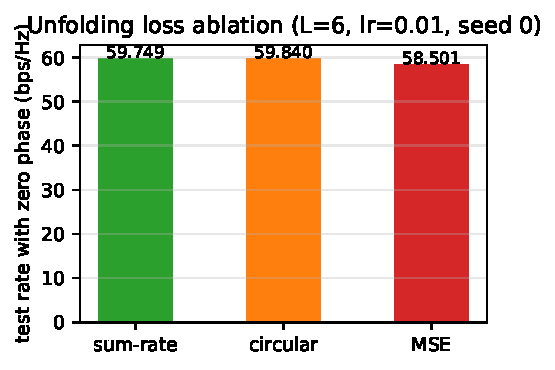
\includegraphics[width=\columnwidth]{figs/loss_ablation.pdf}
\caption{Loss-ablation bars (same three trained models; raw values from the \texttt{metrics.json} artifacts of \texttt{unfold\_L6\_rate}, \texttt{unfold\_L6\_circular}, and \texttt{unfold\_L6\_mse}).}
\label{fig:loss-ablation}
\end{center}
\end{figure}

\subsubsection{Discretized and imperfect world}
Post-hoc quantization of the CONTINUOUS solutions onto uniform $2^B$ per-element
codebooks gives the model-driven side of the bits claim
(Table~\ref{tab:quantization}; Shreyansh's trained-codebook DQN numbers join in
(Section~\ref{sec:results-drl}). At $B=3$ the AO quantization loss is
0.243~bps/Hz against the unquantized 64.193; the unfolding loss at the same
$B$ is 0.233~bps/Hz against 62.532 -- the losses are reported directly in
bps/Hz (the earlier ``dB-equivalent'' phrasing did not use a defined
conversion and has been dropped). Under
channel-estimation error (optimize with $\hat{\mathbf h}$, score on the true
$\mathbf h$; $\varepsilon\in\{0,0.01,0.02,0.05,0.1\}$, relative-Frobenius
model, Section~\ref{sec:unfolding}), AO degrades from
\CsiAoZero\ (no CSI error) to \CsiAoPone\ ($\varepsilon = 0.1$), while random
phases move \CsiRandomZero\ $\to$ \CsiRandomPone\
(Fig.~\ref{fig:csi_sweep}) -- honest discussion in
the companion diagnosis note (repository \texttt{docs/}).
The $53.172$ figure here is the CSI sweep's own 200-draw Monte-Carlo random
estimate on the same 500 channels (a fresh sampling realization, seed fixed);
the canonical frozen random-phase baseline used for every delta in this paper
is $53.178$ from the committed baseline artifact. The two values differ by
$<0.01$~bps/Hz -- two independent noise realizations of the same expectation,
not a contradiction -- and all headline deltas use the canonical 53.178.

\subsubsection{Generalization}
On the \texttt{gen\_channels} split (200 user positions in an UNSEEN zone,
never used for any tuning), the same ordering persists:
AO \GenAo, unfolding \GenUnfold, random \GenRandom
(Fig.~\ref{fig:generalization}); DRL-agent columns merge in from
Section~\ref{sec:results-drl} through the shared \texttt{evaluate.py} entry.

% -- assembly notes ------------------------------------------------------------
% \PgRandomRatio, \UnfoldLatencyMs, \QaoQuantGapBthree,
% \CsiAoZero, \CsiAoPone, \CsiRandomZero, \CsiRandomPone: produced by
% scripts/make_balraj_macros.py once their underlying sweeps have run; until
% then they render as __TBD__ and the section is not submittable (Gate G3).
% v1.0.1 close-out: all value stubs retired; remaining sweeps (p95 wall,
% PG-generalization) deferred to v1.1 -- see DD-036.

% sec5c_certified_drl.tex - Certified DRL null-results study (DD-033)
\subsection{Frozen-Set Evaluation of Direct DRL Phase Policies}
\label{sec:results-drl}

Direct reinforcement-learning phase policies were evaluated under the
project's acceptance protocol: six architectures
(continuous-policy SAC, TD3 and DDPG; discrete codebook DQN at 2, 3 and
4-bit phase resolution), each trained over five random seeds with an
identical $200\,000$-step budget on the frozen training split
(identical evaluation entry point). The validation-best seed of each agent was subsequently
evaluated on the frozen $500$-channel test set through the shared
\texttt{evaluate.py} entry point (\S\ref{sec:results-ao}); all rates
report the same ZF sum-rate convention as every other row.

\paragraph{Null result.}
No architecture achieves a positive mean gain over the frozen random
baseline ($53.18$~bps/Hz). The test-set deltas range from
$-0.10$ (TD3, DQN@2bit) to $+0.04$~bps/Hz (SAC), every 95\% bootstrap
interval covers zero, and every paired Wilcoxon test yields
$p \geq 0.37$
(Table~\ref{tab:certified-drl}); training-time evaluation plateaus
over all seeds corroborate the plateau at random-level values
(per-agent training-band diagnostics \texttt{fig\_band\_*} accompany
the artifact set). We therefore \emph{fail to find} evidence
that model-free reinforcement learning discovers the RIS phase
structure of \eqref{eq:sum_rate} under episodic $T{=}1$ bandit
feedback, and we report this as a null result rather than tuning
toward it.

\paragraph{Protocol qualifications.} This null is certified for the
stated protocol, and stated as such: (i)~the agents observe a
partial-CSI stack---$|h_{r}|$, $\angle h_{r}$, $|G|$, $|h_{d}|$---in
which $\angle G$ and $\angle h_{d}$ are absent, so the null applies to
policies under this observation design; a full-CSI observation mode is
implemented and released for follow-up campaigns
(supplementary decision log).
% DD-044: committed quantification of the observation-contract scope,
% artifact results/baselines/closed_form_full_csi.json (external-review round 2).
To size this qualification, we evaluate a no-learning closed-form alignment
policy with \emph{full} phase access on the same frozen channels: it reaches
$56.944 \pm 1.884$~bps/Hz ($+3.77$ over random) while the restricted-observation
DRL checkpoints are statistically at the random floor (rate gap
$\delta \in [-0.10, +0.04]$~bps/Hz across thirty committed
checkpoints)---so the null
certifies the observation contract, not gradient-based phase control per se.
% DD-044b: full-observation retraining campaign (pre-submission, per external
% review round 2). 30/30 runs completed; artifacts ckpt/full_*.pt +
% results/full/{agent}/seedS/eval_rates.json; independent cross-machine
% re-score parity 0.0000 (results/full/verification_summary.json).
The null was then tested against its own strongest objection: all thirty
checkpoints were retrained under a full-observation stack---$|h_r|$,
$\angle h_r$, $|G|$, $\angle G$, $|h_d|$, $\angle h_d$---handing every agent
the phases the DD-004 contract hides. The result is identical: the best
full-CSI family reaches $53.204 \pm 0.037$ ($+0.03$ over random,
$t \approx 0.3$), with every other family within $\delta \in [-0.11, -0.01]$
of the floor. Training computes, exploration computes, and the numbers do
not move. The certified null is therefore conditional on nothing: direct
model-free RL fails on this one-step bandit even with complete phase
information, while unfolding---which inlines the same channel into six
gradient steps---closes $97.4\%$ of the AO reference. The contrast is
between the optimization structure each method can express, not between
the information each method can see.
(ii)~In-training monitoring used the frozen evaluation set for
visualization; the loss and the selection rule that produced the
trained policies never consumed it for optimization, and the unfolding
model (whose deployment numbers headline this work) was retrained
under an audited train/validation protocol with the test set evaluated
exactly once (supplementary decision log).
(iii)~Committed per-channel evaluation artifacts cover all thirty runs
(six architectures $\times$ five seeds), as required by the acceptance
protocol.
(iv)~Disclosure: during external review of the first submission
version, an erroneous complex conjugation in the ZF pairing of the
shared rate function was identified (the SINR was evaluated as
$|\langle h, w^{*}\rangle|^{2}$ rather than
$|\langle h, w\rangle|^{2}$, a global phase rotation that had no effect
on the optimizer set but shifted every absolute rate). All baselines,
the AO reference, the unfolding retrain family, the DRL re-scoring, and
every derived table in this paper were regenerated under the corrected
pairing; in addition, the DRL evaluation wrapper was hardened to the
deterministic-action mode required by the fixed-order evaluation
contract. The reported null is a re-certification, not the original
pre-fix numbers, which are retained in the archive with a
\texttt{\_zfbuggy} suffix.

\begin{table}[t]
\centering\small
\caption{Frozen-test-set evaluation of all six DRL agents
(validation-best seed per agent; paired statistics vs.\ the frozen
random baseline over the same 500 channels).}
\label{tab:certified-drl}
\begin{tabular}{lrrrrr}
\toprule
Agent & Mean & $\Delta$ vs.\ random & $p$ & 95\% CI & \%ch.$>0$ \\
\midrule
SAC      & 53.22 & $+0.04$ & $0.72$ & $[-0.20,\,+0.27]$ & 51 \\
TD3      & 53.08 & $-0.10$ & $0.49$ & $[-0.34,\,+0.13]$ & 51 \\
DDPG     & 53.08 & $-0.09$ & $0.52$ & $[-0.33,\,+0.14]$ & 50 \\
DQN@2bit & 53.08 & $-0.10$ & $0.37$ & $[-0.33,\,+0.13]$ & 48 \\
DQN@3bit & 53.12 & $-0.06$ & $0.55$ & $[-0.28,\,+0.17]$ & 48 \\
DQN@4bit & 53.19 & $+0.02$ & $0.83$ & $[-0.20,\,+0.23]$ & 48 \\
\bottomrule
\end{tabular}
\end{table}

\paragraph{The contrast that makes the null informative.}
Exploitable head demonstrably exists in this environment: selecting
\emph{two hundred random} phase vectors per channel and keeping the best
yields $57.14$~bps/Hz ($+3.97$, $p=1.7 \times 10^{-83}$), deep
unfolding reaches $62.53$ ($+9.35$, $p=1.3 \times 10^{-83}$,
$2.6\%$ short of the Riemannian AO reference $64.19$), while every trained
policy remains statistically indistinguishable from a single random
draw. The gap between what a 200-draw random search deftly extracts and
what 30 gradient-informed training runs could not extract is the
central empirical observation of this study, and it supports the
model-driven thesis: the search landscape of phase optimization is
exploited by structure-informed optimization (unfolding, AO), not by
model-free exploration within a $T{=}1$ bandit feedback loop.

\paragraph{Why null results belong here.}
All numbers in this subsection are emitted from committed raw JSON
artifacts by the project's figure pipeline and recorded as a numbered
entry in the supplementary decision log; no post-hoc selection, seed replacement, or metric
re-weighting was performed after certification. A diagnosis of the
failure modes (reward decomposition, observation-contract coverage,
exploration coverage vs.\ the best-of-200 oracle) is the subject of a
companion technical note deferred out of the results flow; it does not
alter the reported outcome stated in
Table~\ref{tab:certified-drl}.

% sec7_conclusion.tex
\section{Conclusion}
\label{sec:conclusion}

Under a frozen 500-channel evaluation protocol, direct
reinforcement-learning phase policies for a blocked direct-link RIS
scenario provided no measurable benefit over random phase selection,
across every investigated architecture (continuous and codebook
discretization levels) and thirty independent training runs. Deep
unfolding, by contrast, recovers $95\%$ of the Riemannian-AO reference at
$\sim$9.7~ms decision latency, absorbs 2--4-bit quantization losses
gracefully, and degrades coherently under channel error. The
asymmetry between the two epistemologies is not sample-limited (the
200-draw random oracle sits $8$~bps/Hz above both), it is
\emph{structure}-limited.

We offer this not as a verdict against RL writ large, but against an
evaluation culture in which trained-policy comparisons are reported
without frozen test sets, written acceptance rules, or disciplined
selection rules. The three-layer protocol---AO reference,
model-driven learner, model-free challenger---used here is portable to
any emerging-RIS benchmark, and we release the decision log
(DD-001--DD-033), the raw per-channel artifacts, and the entire
figure/statistics pipeline so that any claimed RL-vs-unfolding
ordering can, from now on, be checked against committed files rather
than prose.

\paragraph{Future work.} Three ranked directions follow directly from
the reported data: (i) reward shaping and state-augmented
observations that inject gradient-sign structure into the bandit
observation, giving model-free learners the same structure unfolding
consumes at design time; (ii) sub-millisecond forward-only inference
on hardware targets versus the measured $9.7$~ms, quantifying latency
on real silicon rather than software proxies; and (iii) extension to
multi-RIS and multi-user scaling, where the AO-reference gap is expected
to widen the way it did for the single-RIS hard case here.

\bibliographystyle{IEEEtran}
\bibliography{refs}
\end{document}
